% File: intro.tex
% Date: Sun Aug 26 22:09:02 2012 +0800
% Author: Yuxin Wu <ppwwyyxxc@gmail.com>
\section{Introduction}

\begin{enumerate}
	\item 编译:  
		程序共有四个版本,分别为串行,MPI,OpenMP,pthread.需通过改变环境变量\verb|DEFINES|分别编译.源码中提供了一个脚本\verb|make_all_version|可以一次性编译出四个可执行文件.
		编译并行版本的环境变量分别为\verb|DEFINES=-DUSE_OMP, -DUSE_MPI, -DUSE_PTHREAD|,单独编译出的可执行文件为\verb|main|
\begin{lstlisting}
$ ./make_all_version
make seq verson ...
done
make omp version ...
done
make pthread version ...
done
make mpi version ...
done
$ DEFINES=-DUSE_OMP make
mkdir: created directory ‘obj’
[dep] ./calculate.cc ...
[dep] ./main.cc ...
[dep] ./Xoutput.cc ...
[dep] ./png_writer.cc ...
[cc] calculate.cc ...
[cc] Xoutput.cc ...
[cc] main.cc ...
[cc] png_writer.cc ...
Linking ...
$
\end{lstlisting}

\item 命令行参数:
	\begin{lstlisting}[basicstyle=\scriptsize\ttfamily]
$ ./main
Options:
  --nproc=NUM, -n      number of threads(pthread only). number of CPUs by default
  --size=SIZE, -s      size of picture. SIZE is of format `<width>x<height>'
                       eg. `800x800' (default), 
  --domain=DOMAIN, -d  plotting domain. DOMAIN is of format 
                       `<xmin>,<ymin>,<width>,<height>', where x and y are 
                       the coordinates of left-bottom corner.
                       eg. `-2,-2,4,4` (default).
  --iter=NUM, -i       set max number of iteration of function. 1000 by default.
  --png=FILENAME, -p   save image to png file.
  --X, -x                              use X to show image. can move and zoom image.
  --help, -h           show this help and quit
\end{lstlisting}
程序支持如下的命令行参数:
\begin{description}
	\item \verb|--nproc=NUM|指定pthread使用的线程数量,对其他多线程模式无效.
	\item \verb|--size=SIZE|指定生成图片的大小.
	\item \verb|--domain=DOMAIN|指定绘图区域的坐标.
	\item \verb|--iter=NUM|指定计算时的迭代次数.
	\item \verb|--png=FILE|将结果输出到png文件中.
	\item \verb|--X|将图片用Xlib显示.
	\item \verb|--help|输出帮助信息.
\end{description}


\item 测试运行:
\begin{lstlisting}
$ ./omp -s 2000x2000
0.206523 seconds elapsed
$ ./pthread -s 2000x2000
0.199212 seconds elapsed
$ mpirun -n 4 ./mpi  -s 2000x2000
0.254203 seconds elapsed
$ ./seq -s 2000x2000
0.653799 seconds elapsed
$ 
\end{lstlisting}

\item 界面展示:
	\begin{lstlisting}
	$ ./pthread -x
	0.035687 seconds elapsed
	$ 
	\end{lstlisting}

	\begin{figure}[H]
		\centering
		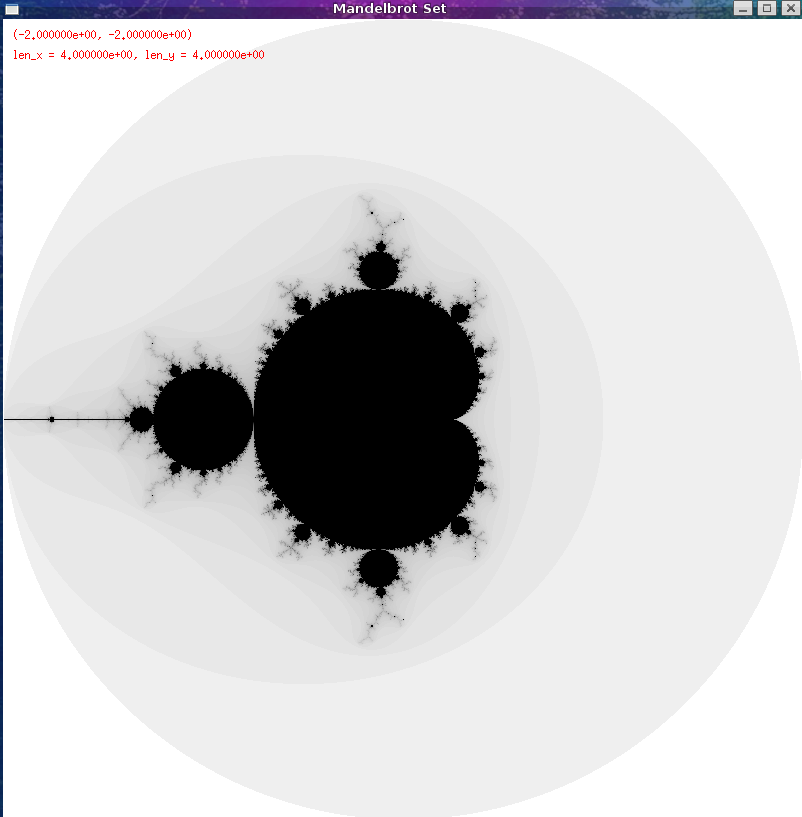
\includegraphics[scale=0.4]{res/show.png}
	\end{figure}

	在X窗口中,可使用方向键移动屏幕,用``=''/``-''进行放大/缩小(由于精度限制,只能放大约$ 10^{15}$倍),用鼠标左右键改变区域中心再放大/缩小,s让程序从\verb|stdin|接收文件名并截图保存,
	c键从\verb|stdin|接受新的迭代次数取值,以观察同一位置在不同迭代次数下的不同图形.ESC键退出.

	窗口左上角显示的是窗口左下角坐标以及窗口在$ x,y$方向上跨越的坐标系上的长度.



\end{enumerate}
